% Standalone source for Figure: system architecture.
% Compile with: pdflatex architecture.tex  (produces architecture.pdf)
\documentclass[tikz,border=4pt]{standalone}
\usepackage{amsmath,amssymb}
\usetikzlibrary{positioning,arrows.meta,fit,backgrounds,calc}
\definecolor{blue1}{HTML}{2A78D6}
\definecolor{orange1}{HTML}{EB6834}
\definecolor{aqua1}{HTML}{1BAF7A}
\definecolor{ink2}{HTML}{52514E}
\begin{document}
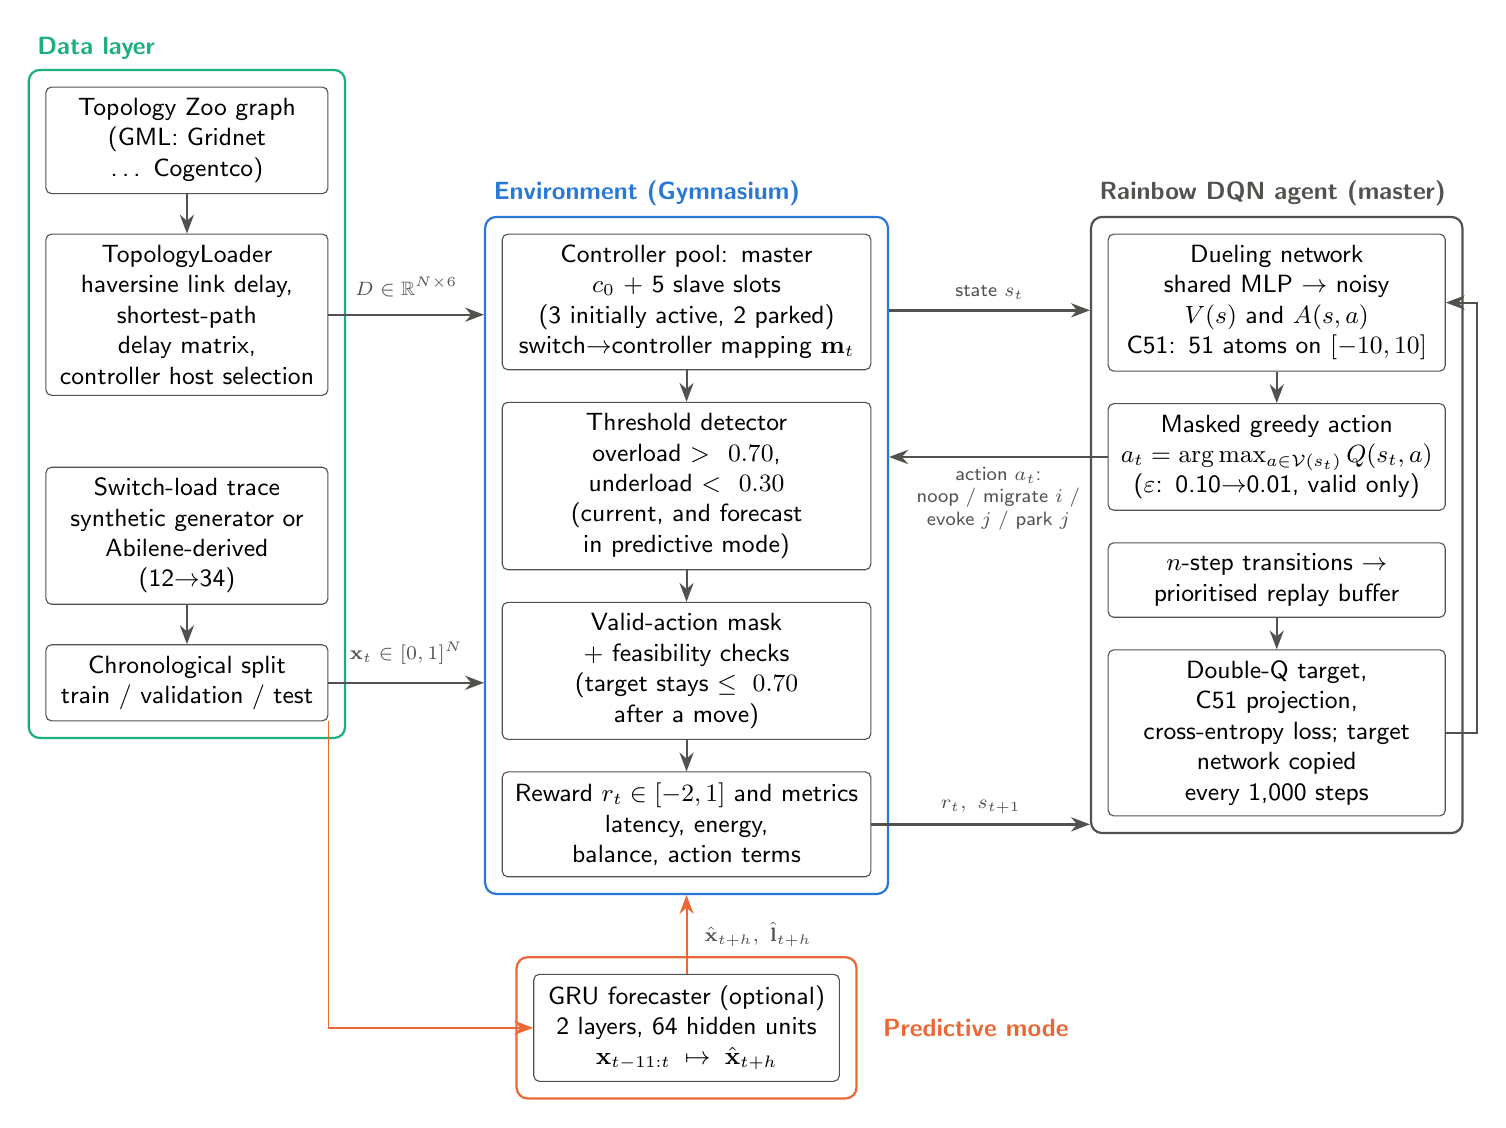
\begin{tikzpicture}[
  font=\sffamily\small,
  every node/.append style={execute at begin node={\hyphenpenalty 10000\relax}},
  box/.style={draw=ink2, rounded corners=2pt, align=center, fill=white,
              minimum height=9mm, inner sep=4pt, text width=#1},
  box/.default=33mm,
  grp/.style={draw=#1, rounded corners=4pt, line width=0.8pt, inner sep=6pt},
  lbl/.style={font=\sffamily\bfseries\small, anchor=south west},
  arr/.style={-{Stealth[length=2.4mm]}, line width=0.7pt, draw=ink2},
  note/.style={font=\sffamily\scriptsize, text=ink2, align=center},
]
% ---------------- data layer
\node[box] (gml) {Topology Zoo graph\\(GML: Gridnet \ldots\ Cogentco)};
\node[box, below=5mm of gml] (topo) {TopologyLoader\\haversine link delay,\\shortest-path delay matrix,\\controller host selection};
\node[box, below=9mm of topo] (trace) {Switch-load trace\\synthetic generator or\\Abilene-derived (12$\rightarrow$34)};
\node[box, below=5mm of trace] (split) {Chronological split\\train / validation / test};
\draw[arr] (gml) -- (topo);
\draw[arr] (trace) -- (split);
\begin{scope}[on background layer]
  \node[grp=aqua1, fit=(gml)(topo)(trace)(split)] (data) {};
\end{scope}
\node[lbl, text=aqua1] at (data.north west) {Data layer};

% ---------------- environment
\node[box=44mm, right=22mm of topo.north east, anchor=north west] (pool)
  {Controller pool: master $c_0$ + 5 slave slots\\(3 initially active, 2 parked)\\switch$\rightarrow$controller mapping $\mathbf{m}_t$};
\node[box=44mm, below=4mm of pool] (thr)
  {Threshold detector\\overload $>0.70$, underload $<0.30$\\(current, and forecast in predictive mode)};
\node[box=44mm, below=4mm of thr] (mask)
  {Valid-action mask + feasibility checks\\(target stays $\le0.70$ after a move)};
\node[box=44mm, below=4mm of mask] (rew)
  {Reward $r_t\in[-2,1]$ and metrics\\latency, energy, balance, action terms};
\draw[arr] (pool) -- (thr);
\draw[arr] (thr) -- (mask);
\draw[arr] (mask) -- (rew);
\begin{scope}[on background layer]
  \node[grp=blue1, fit=(pool)(thr)(mask)(rew)] (env) {};
\end{scope}
\node[lbl, text=blue1] at (env.north west) {Environment (Gymnasium)};

\draw[arr] (topo.east) -- node[note, above, pos=0.5, yshift=1mm] {$D\in\mathbb{R}^{N\times6}$} (topo.east -| env.west);
\draw[arr] (split.east) -- node[note, above, pos=0.5, yshift=1mm] {$\mathbf{x}_t\in[0,1]^N$} (split.east -| env.west);

% ---------------- GRU
\node[box=36mm, below=10mm of env.south] (gru)
  {GRU forecaster (optional)\\2 layers, 64 hidden units\\$\mathbf{x}_{t-11:t}\mapsto\hat{\mathbf{x}}_{t+h}$};
\begin{scope}[on background layer]
  \node[grp=orange1, fit=(gru)] (gruG) {};
\end{scope}
\node[lbl, text=orange1, anchor=west] at ([xshift=2mm]gruG.east) {Predictive mode};
\draw[arr, draw=orange1] (split.south east) |- ($(gru.west)+(0,0)$);
\draw[arr, draw=orange1] (gru.north) -- node[note, right, xshift=1mm] {$\hat{\mathbf{x}}_{t+h},\ \hat{\mathbf{l}}_{t+h}$} (gru.north |- env.south);

% ---------------- agent
\node[box=40mm, right=30mm of pool.north east, anchor=north west] (net)
  {Dueling network\\shared MLP $\rightarrow$ noisy $V(s)$ and $A(s,a)$\\C51: 51 atoms on $[-10,10]$};
\node[box=40mm, below=4mm of net] (sel)
  {Masked greedy action\\$a_t=\arg\max_{a\in\mathcal{V}(s_t)}Q(s_t,a)$\\($\varepsilon$: 0.10$\rightarrow$0.01, valid only)};
\node[box=40mm, below=4mm of sel] (per)
  {$n$-step transitions $\rightarrow$\\prioritised replay buffer};
\node[box=40mm, below=4mm of per] (upd)
  {Double-Q target, C51 projection,\\cross-entropy loss; target\\network copied every 1,000 steps};
\draw[arr] (net) -- (sel);
\draw[arr] (per) -- (upd);
\draw[arr] (upd.east) -- ++(4mm,0) |- (net.east);
\begin{scope}[on background layer]
  \node[grp=ink2, fit=(net)(sel)(per)(upd)] (agent) {};
\end{scope}
\node[lbl, text=ink2] at (agent.north west) {Rainbow DQN agent (master)};

% ---------------- interaction
\draw[arr, line width=1pt] (env.north east) ++(0,-12mm) coordinate (s1) -- node[note, above] {state $s_t$} (s1 -| agent.west);
\draw[arr, line width=1pt] (sel.west) -- node[note, below, align=center] {action $a_t$:\\noop / migrate $i$ /\\evoke $j$ / park $j$} (sel.west -| env.east);
\draw[arr, line width=1pt] (rew.east) -- node[note, above] {$r_t,\ s_{t+1}$} (rew.east -| agent.west);
\end{tikzpicture}
\end{document}
